\documentclass{article}

\usepackage{tikz}
\usepackage{pdfpages}
\usepackage{parskip}
\usepackage{amsmath}
\usepackage[margin=.6in]{geometry}

\begin{document}
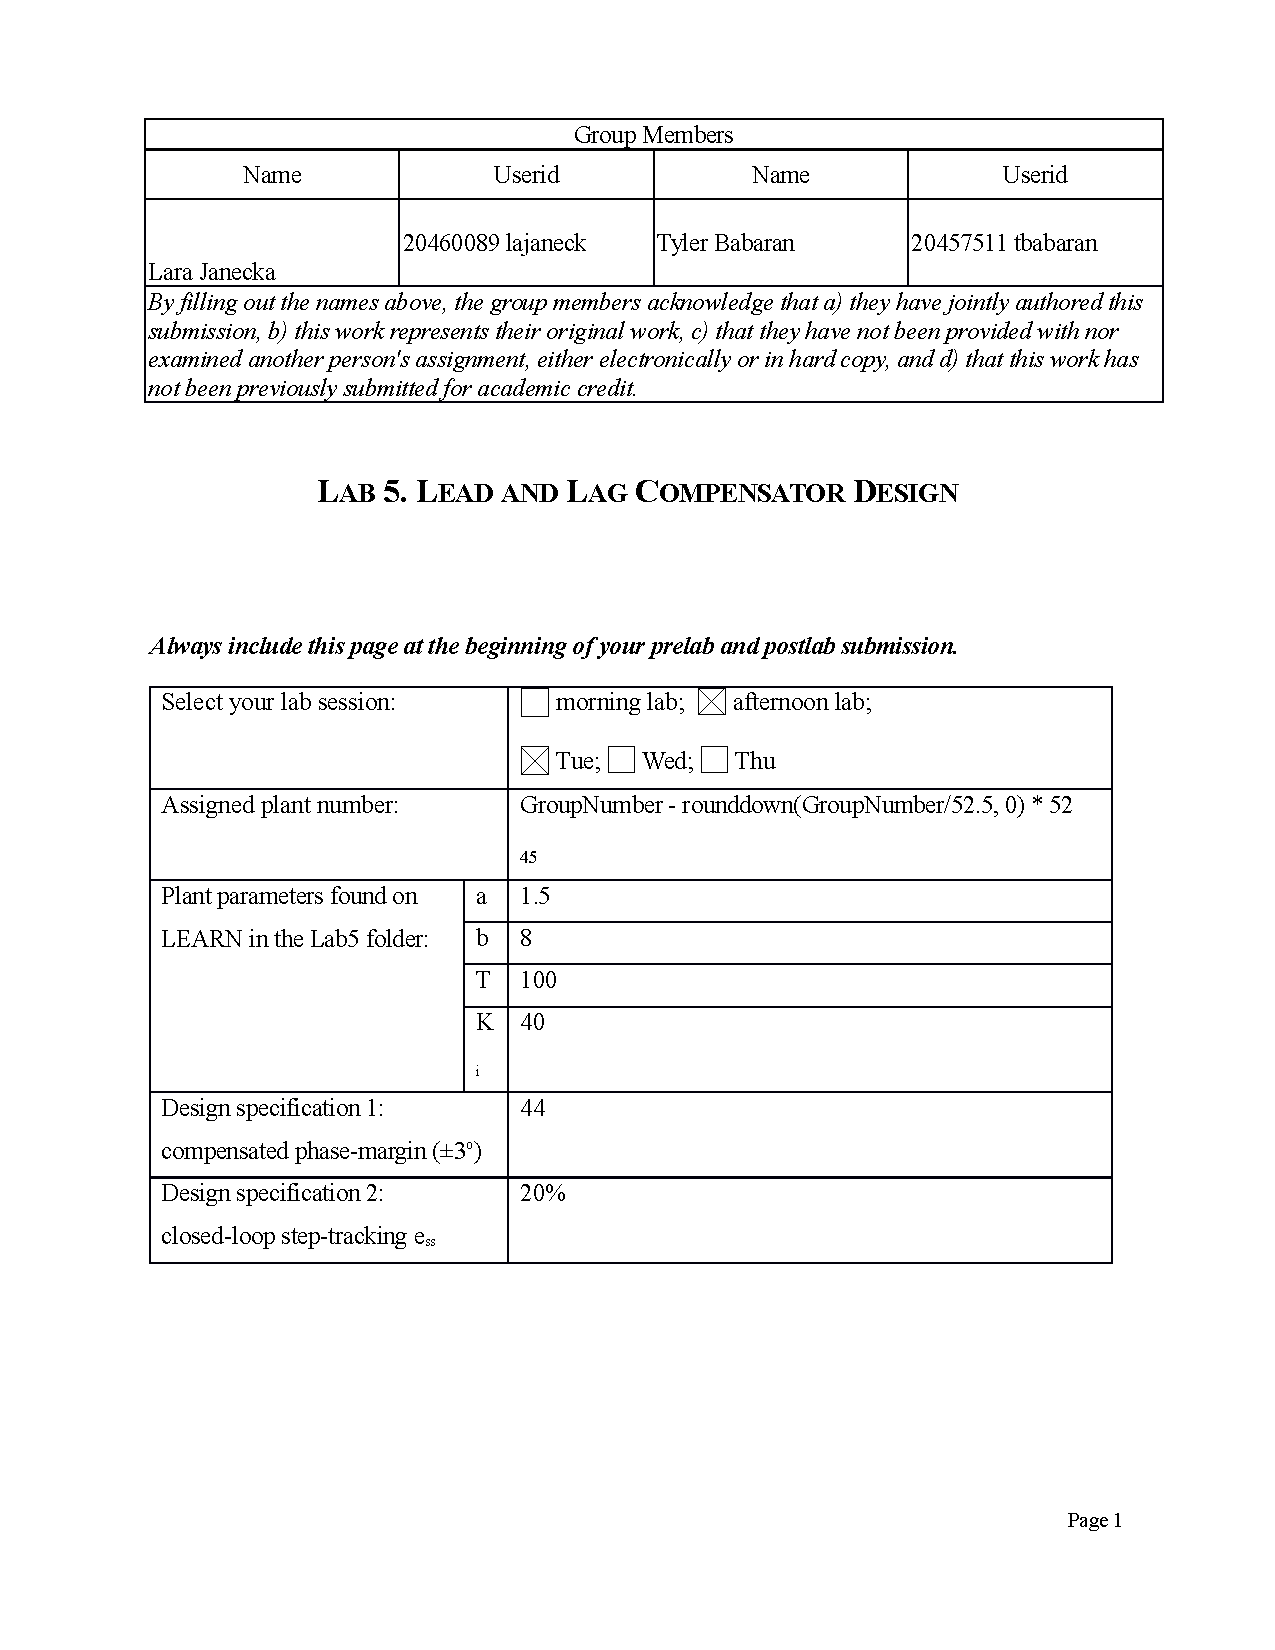
\includepdf[pages={1}]{page1.pdf}


\begin{table}[!htbp]
\centering
    \begin{tabular}{|c|c|c|c|}
        \hline
        &  Calculated & Experimental & Error \\
        \hline
        \textbf{Natural Frequency} & 178.89 & - & -\\
        \hline
        \textbf{Time to First Peak} & 0.019 & 0.019 & 0\\
        \hline
        \textbf{Overshoot} & 23 & 18 & 21\\
        \hline
    \end{tabular}
    \caption{Verification data for P(s)}
\end{table}

\begin{figure}[!htbp]
    \centering
    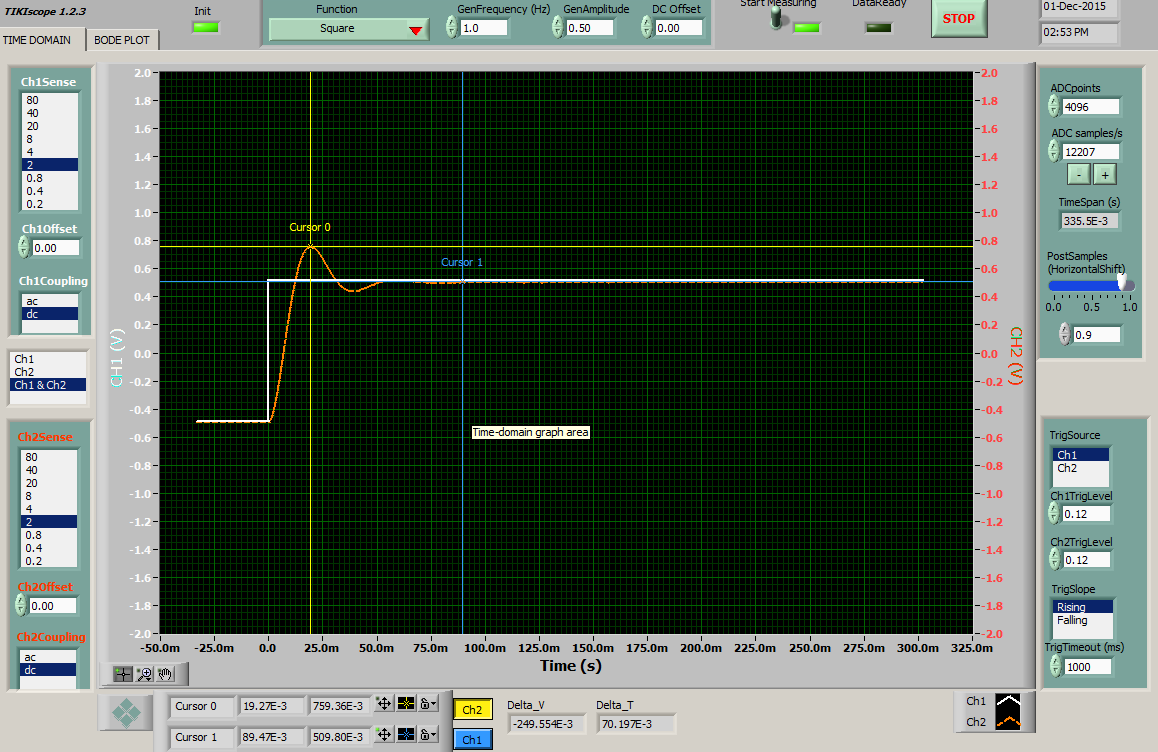
\includegraphics[width=0.95\textwidth]{plant_step.png}
    \caption{Plant verification response}
\end{figure}

\newpage
\section{Question 1} % (fold)
\label{sec:question_1}
We did not have to revise our prelab values.
\begin{align*}
\text{C(S)} &= 4\frac{\frac{s}{27.48} + 1}{\frac{s}{12.82} + 1}\\
\end{align*}

These values (with small rounding errors) produced the below images.

\begin{figure}[!htbp]
    \centering
    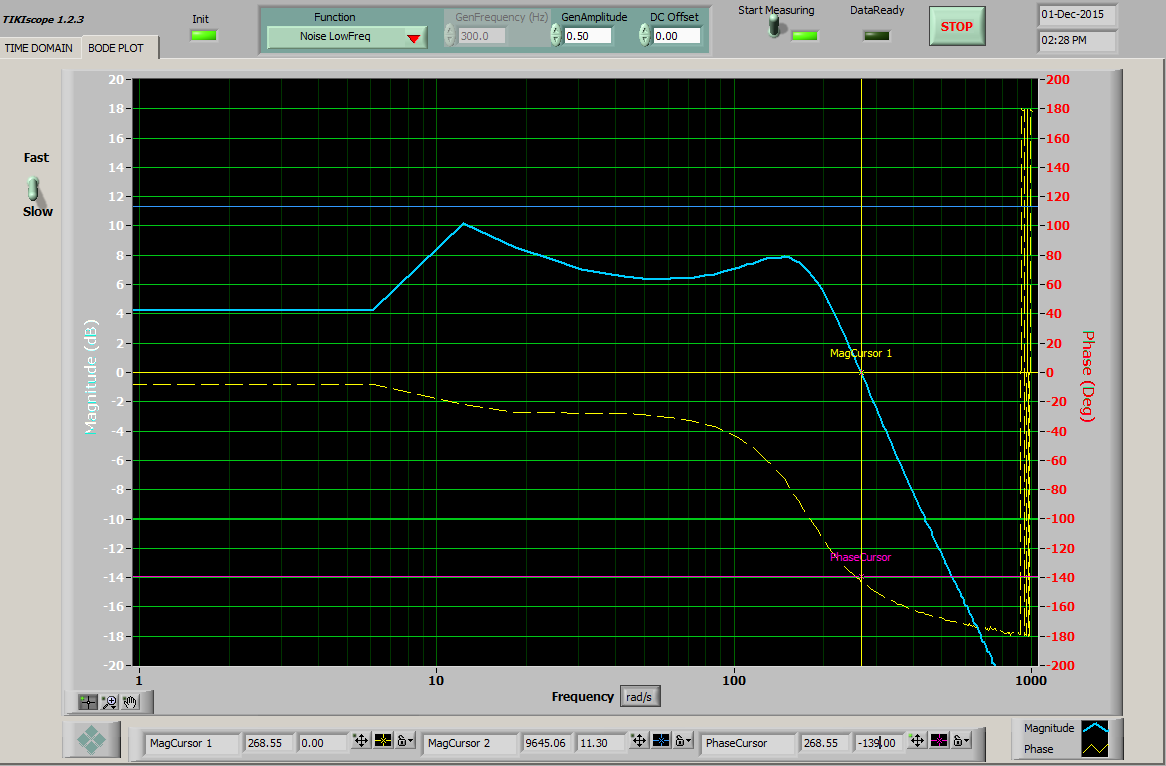
\includegraphics[width=0.95\textwidth]{lag_bode.png}
    \caption{Lag Bode Plot}
\end{figure}

\newpage
\begin{figure}[!htbp]
    \centering
    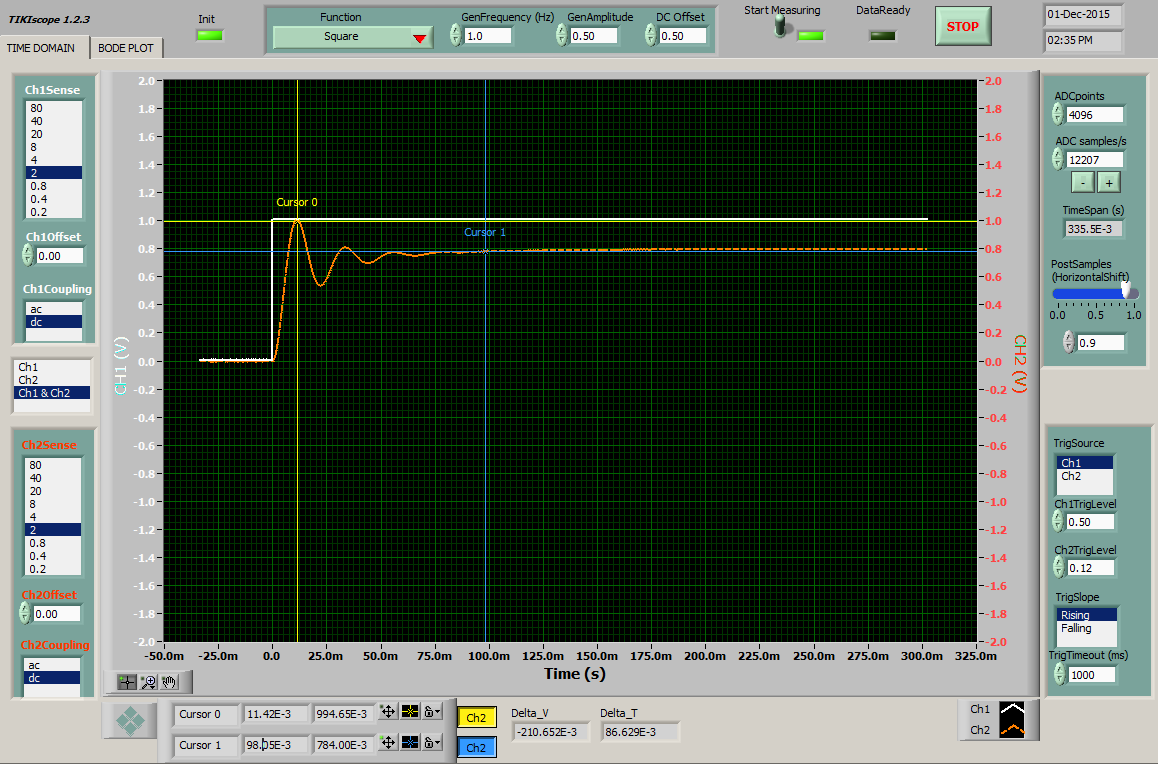
\includegraphics[width=0.95\textwidth]{lag_step.png}
    \caption{Lag Step Response}
\end{figure}

% section question_1 (end)


\newpage
\section{Question 2} % (fold)
\label{sec:question_2}
We did not have to revise our prelab values.
\begin{align*}
\text{C(S)} &= 4\frac{\frac{s}{252.3} + 1}{\frac{s}{602.41} + 1}\\
\end{align*}

These values (with small rounding errors) produced the below images.

\begin{figure}[!htbp]
    \centering
    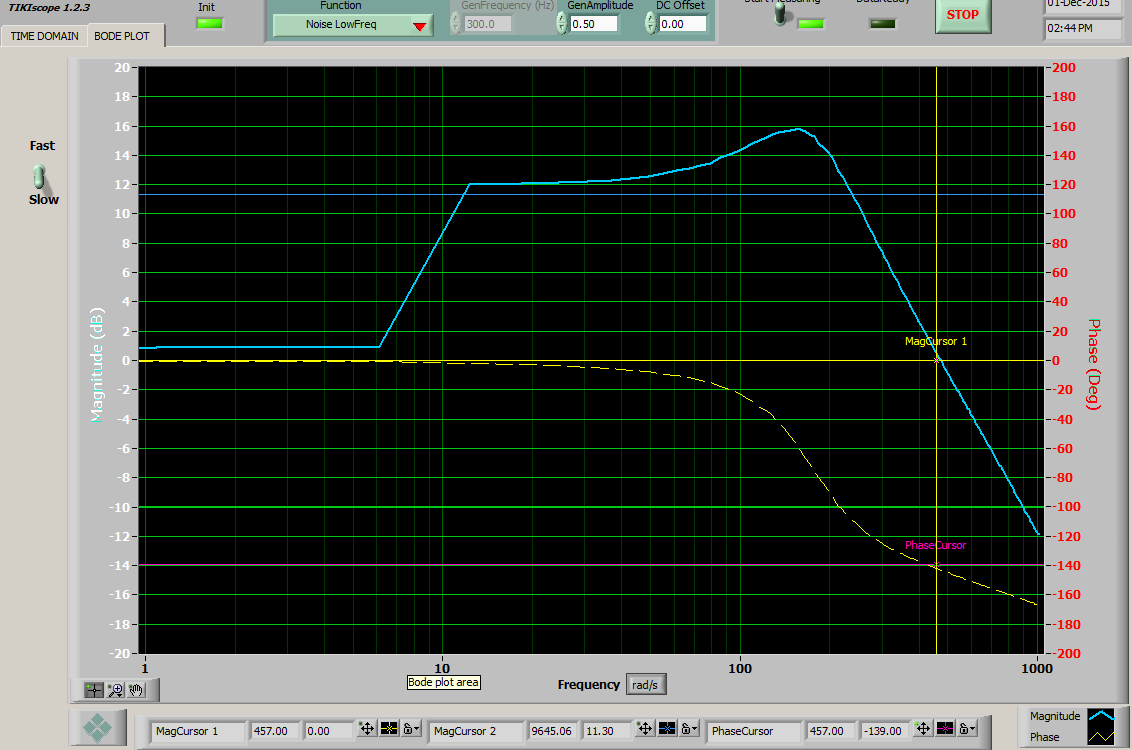
\includegraphics[width=0.95\textwidth]{lead_bode.png}
    \caption{Lead Bode Plot}
\end{figure}

\newpage
\begin{figure}[!htbp]
    \centering
    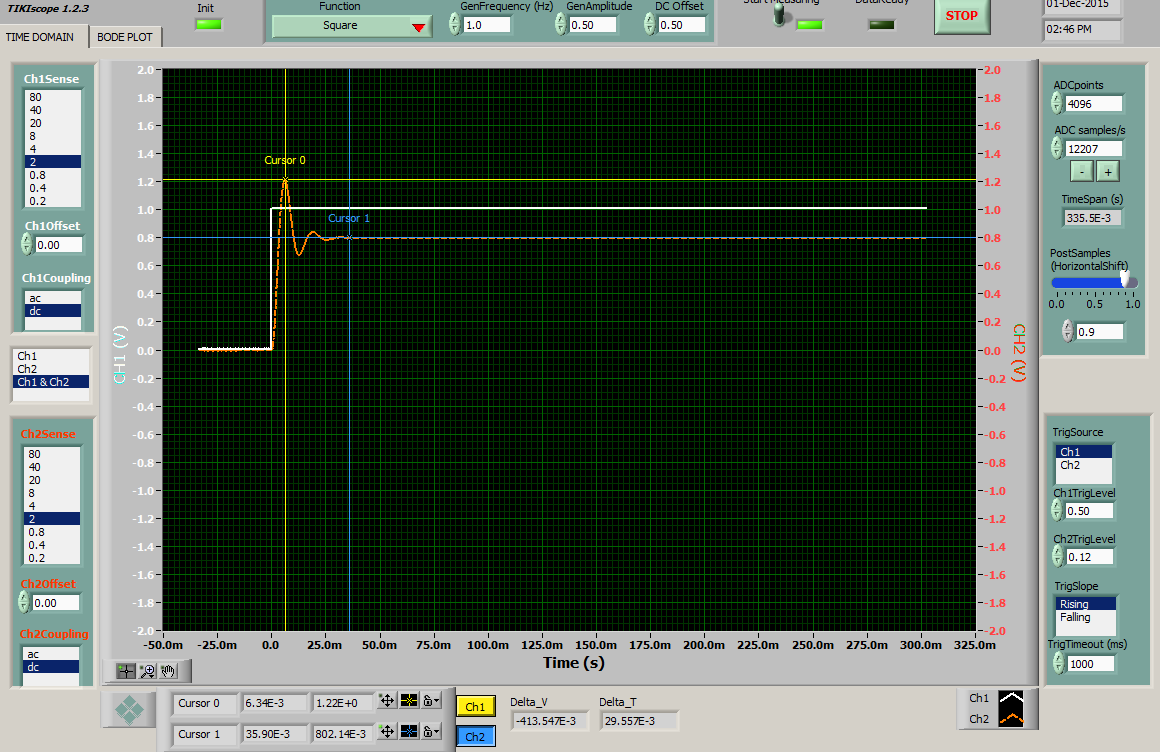
\includegraphics[width=0.95\textwidth]{lead_step.png}
    \caption{Lead Step Response}
\end{figure}

% section question_2 (end)
\newpage
\section{Question 3} % (fold)
\label{sec:question_3}

\begin{table}[!htbp]
\centering
    \begin{tabular}{|c|c|c|}
        \hline
        &  Lag & Lead \\
        \hline
        \textbf{Height of First Peak} & 0.995 & 1.22\\
        \hline
        \textbf{Time to First Peak} & 0.011 & 0.006\\
        \hline
        \textbf{Overshoot} & 21 & 52\\
        \hline
        \textbf{Settling time} & 0.098 & 0.035\\
        \hline
        \textbf{Steady State Error} & 21 & 20\\
        \hline
        \textbf{Low Frequency Gain} & 4 & 0.8\\
        \hline
    \end{tabular}
    \caption{Data for trends}
\end{table}

This table shows that the lag compensator is much slower (resulting in a larger settling time) than the lead compensator but has lower overshoot (resulting in a lower height of first peak). Both compensators achieved the correct steady state error and phase margins (within small error windows).

% section question_3 (end)

\section{Question 4} % (fold)
\label{sec:question_4}
The lag compensator improves the steady state error without making the system become unstable because it does not effect the overshoot (the overshoot for the lag compensated system is almost the same as the overshoot for the uncompensated system).
% section question_4 (end)

\section{Question 5} % (fold)
\label{sec:question_5}
\subsection{a)} % (fold)
\label{sub:a_}
The phase margin when designing the lag compensated system is increased by five degrees to account for lag compensators not being ideal.
\begin{figure}[!htbp]
    \centering
    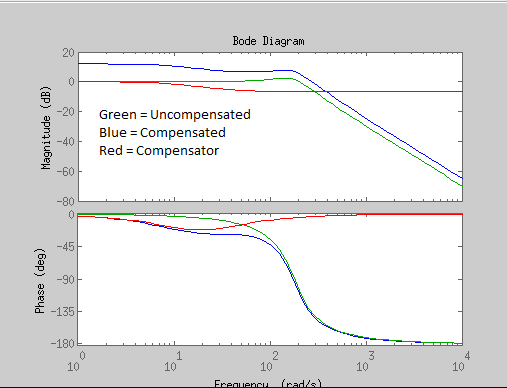
\includegraphics[width=0.95\textwidth]{lag_overlays.png}
    \caption{Lag System Overlays}
\end{figure}
As can be seen in the above image the dip in the phase of the lag compensator now lines up with how we want to shift the cross over frequency of the uncompensated system to shift to fit the desired phase margin.

% subsection a_ (end)
\newpage
\subsection{b)} % (fold)
\label{sub:b_}
The phase margin when designing the lag compensated system is increased by five degrees to account for lead compensators not being ideal.
\begin{figure}[!htbp]
    \centering
    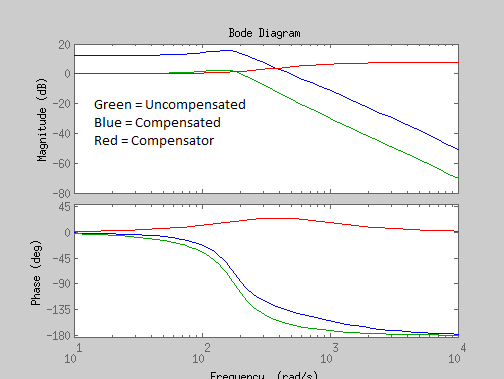
\includegraphics[width=0.95\textwidth]{lead_overlays.png}
    \caption{Lead System Overlays}
\end{figure}
The above image shows the crest of the phase of the lead compensator lining up with how we want to shift the phase of the uncompensated system to match the desired phase margin.


% subsection b_ (end)

% section question_5 (end)

\section{Question 6} % (fold)
\label{sec:question_6}
The lead compensator speeds up the response of a system as seen by its decreased settling time and time to first peak.
% section question_6 (end)
\end{document}
